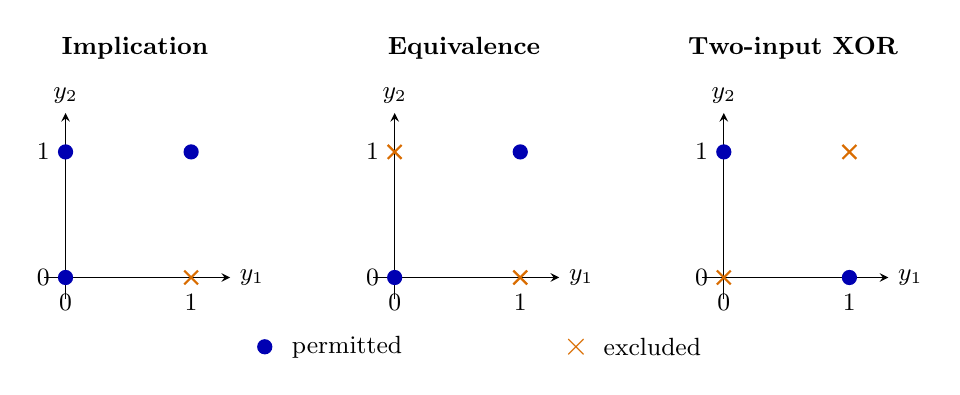
\begin{tikzpicture}[>=stealth,scale=1.1]
\foreach \s/\title in {0/Implication,3.8/Equivalence,7.6/Two-input XOR}{
\begin{scope}[xshift=\s cm]
\node[font=\small\bfseries] at (.8,2.65){\title};
\draw[->,black](-.25,0)--(1.9,0)node[right,font=\small]{$y_1$};
\draw[->,black](0,-.25)--(0,1.9)node[above,font=\small]{$y_2$};
\foreach \v in {0,1}{\node[below,font=\small]at(1.45*\v,-.08){\v};\node[left,font=\small]at(-.07,1.45*\v){\v};}
\end{scope}}
\foreach \s/\a/\b in {0/0/0,0/0/1,0/1/1,3.8/0/0,3.8/1/1,7.6/0/1,7.6/1/0}{\fill[blue!70!black](\s+1.45*\a,1.45*\b)circle(2.5pt);}
\foreach \s/\a/\b in {0/1/0,3.8/0/1,3.8/1/0,7.6/0/0,7.6/1/1}{\draw[orange!85!black,thick](\s+1.45*\a-.08,1.45*\b-.08)--++(.16,.16);\draw[orange!85!black,thick](\s+1.45*\a-.08,1.45*\b+.08)--++(.16,-.16);}
\fill[blue!70!black](2.3,-.8)circle(2.5pt);\node[right,font=\small]at(2.5,-.8){permitted};
\node[orange!85!black,font=\large]at(5.9,-.8){$\times$};\node[right,font=\small]at(6.1,-.8){excluded};
\end{tikzpicture}
